

% Pacotes recomendados no preâmbulo:
% \usepackage{graphicx}
% \usepackage{float}
% \usepackage{booktabs}
% \usepackage{longtable}
% \usepackage{pdflscape}

\begin{table}[H]
\centering
\caption{Resumo exploratório da variável alvo.}
\label{tab:resumo-target-main}
\begin{table}
\caption{Resumo exploratório da variável alvo.}
\label{tab:resumo-target}
\begin{tabular}{lll}
\toprule
Métrica & Valor & Descrição \\
\midrule
Total de observações & 283726 & Quantidade total de registros válidos no target. \\
Não fraudes & 283253 & 99.833290\% da base. \\
Fraudes & 473 & 0.166710\% da base. \\
Classe majoritária & Não Fraude & 283.253 observações. \\
Classe minoritária & Fraude & 473 observações. \\
Razão de desbalanceamento & 598.843552 & Razão entre classe majoritária e classe minoritária. \\
Probabilidade empírica de fraude & 0.0016671014 & Equivalente a 0.166710\%. \\
Entropia de Shannon & 0.0177878619 & Incerteza da distribuição binária do target. \\
Entropia de Shannon normalizada & 0.0177878619 & Entropia dividida pela entropia máxima possível para duas classes. \\
\bottomrule
\end{tabular}
\end{table}

\end{table}

\begin{table}[H]
\centering
\caption{Distribuição absoluta e relativa das classes do target.}
\label{tab:distribuicao-target-main}
\begin{table}
\caption{Distribuição absoluta e relativa das classes do target.}
\label{tab:distribuicao-target}
\begin{tabular}{lrl}
\toprule
Classe & Quantidade & Percentual \\
\midrule
Não Fraude & 283253 & 99.833290 \\
Fraude & 473 & 0.166710 \\
\bottomrule
\end{tabular}
\end{table}

\end{table}

\begin{table}[H]
\centering
\caption{Matrizes de confusão dos cenários de referência.}
\label{tab:matrizes-baseline-target-main}
\begin{table}
\caption{Matrizes de confusão dos cenários de referência para o target.}
\label{tab:matrizes-baseline-target}
\begin{tabular}{lrrrr}
\toprule
Cenário & TN & FP & FN & TP \\
\midrule
Ideal & 283253 & 0 & 0 & 473 \\
Tudo como Não Fraude & 283253 & 0 & 473 & 0 \\
Tudo como Fraude & 0 & 283253 & 0 & 473 \\
\bottomrule
\end{tabular}
\end{table}

\end{table}

\begin{figure}[H]
\centering
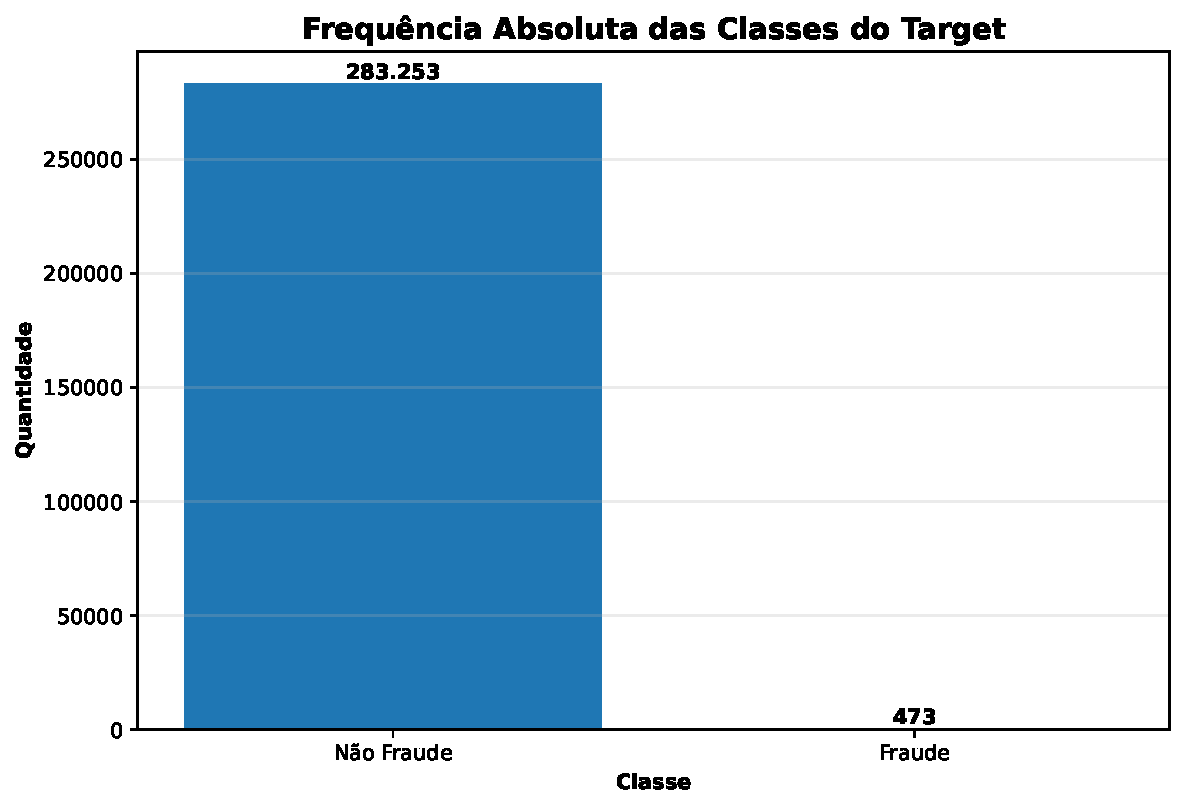
\includegraphics[width=0.75\textwidth]{relatorio_target/grafico_frequencia_absoluta.pdf}
\caption{Frequência absoluta das classes do target.}
\label{fig:target-freq-absoluta}
\end{figure}

\begin{figure}[H]
\centering
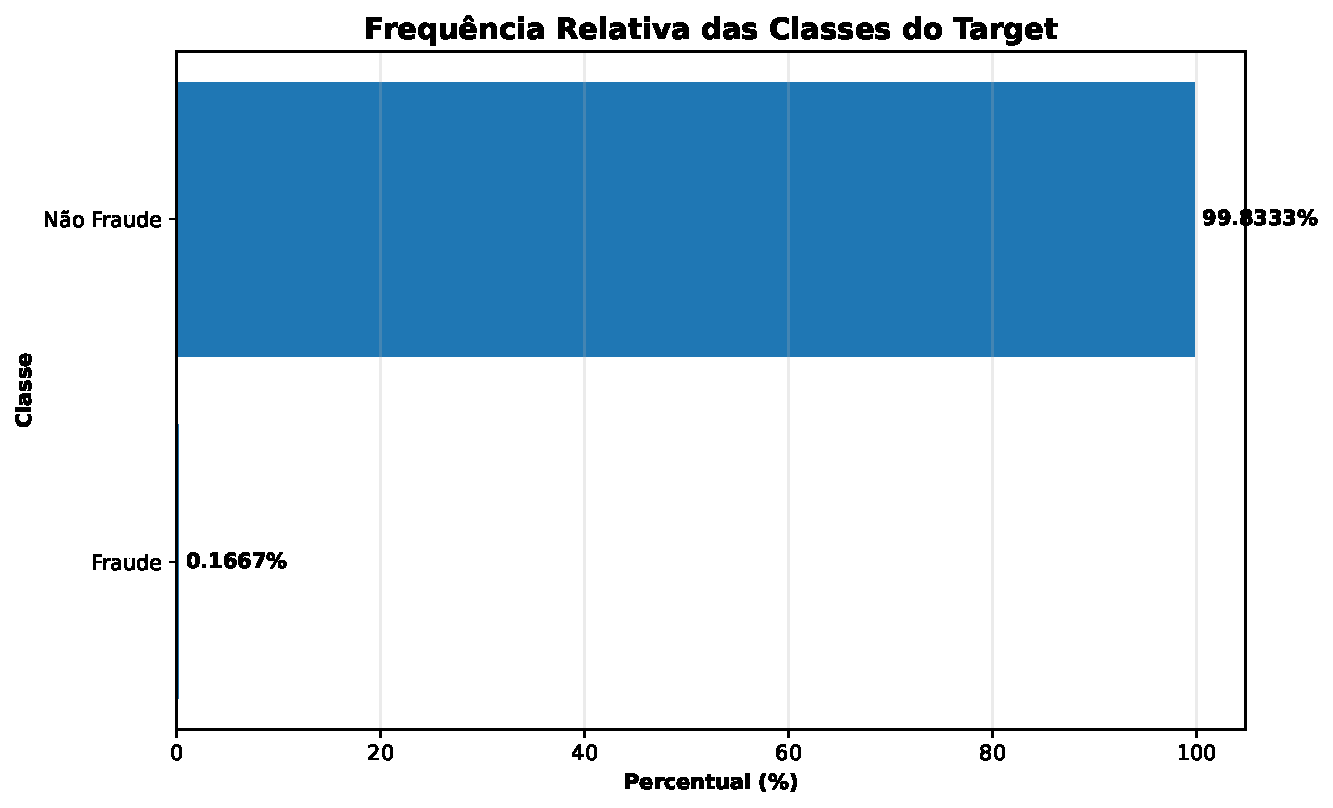
\includegraphics[width=0.75\textwidth]{relatorio_target/grafico_frequencia_relativa.pdf}
\caption{Frequência relativa das classes do target.}
\label{fig:target-freq-relativa}
\end{figure}

\begin{figure}[H]
\centering
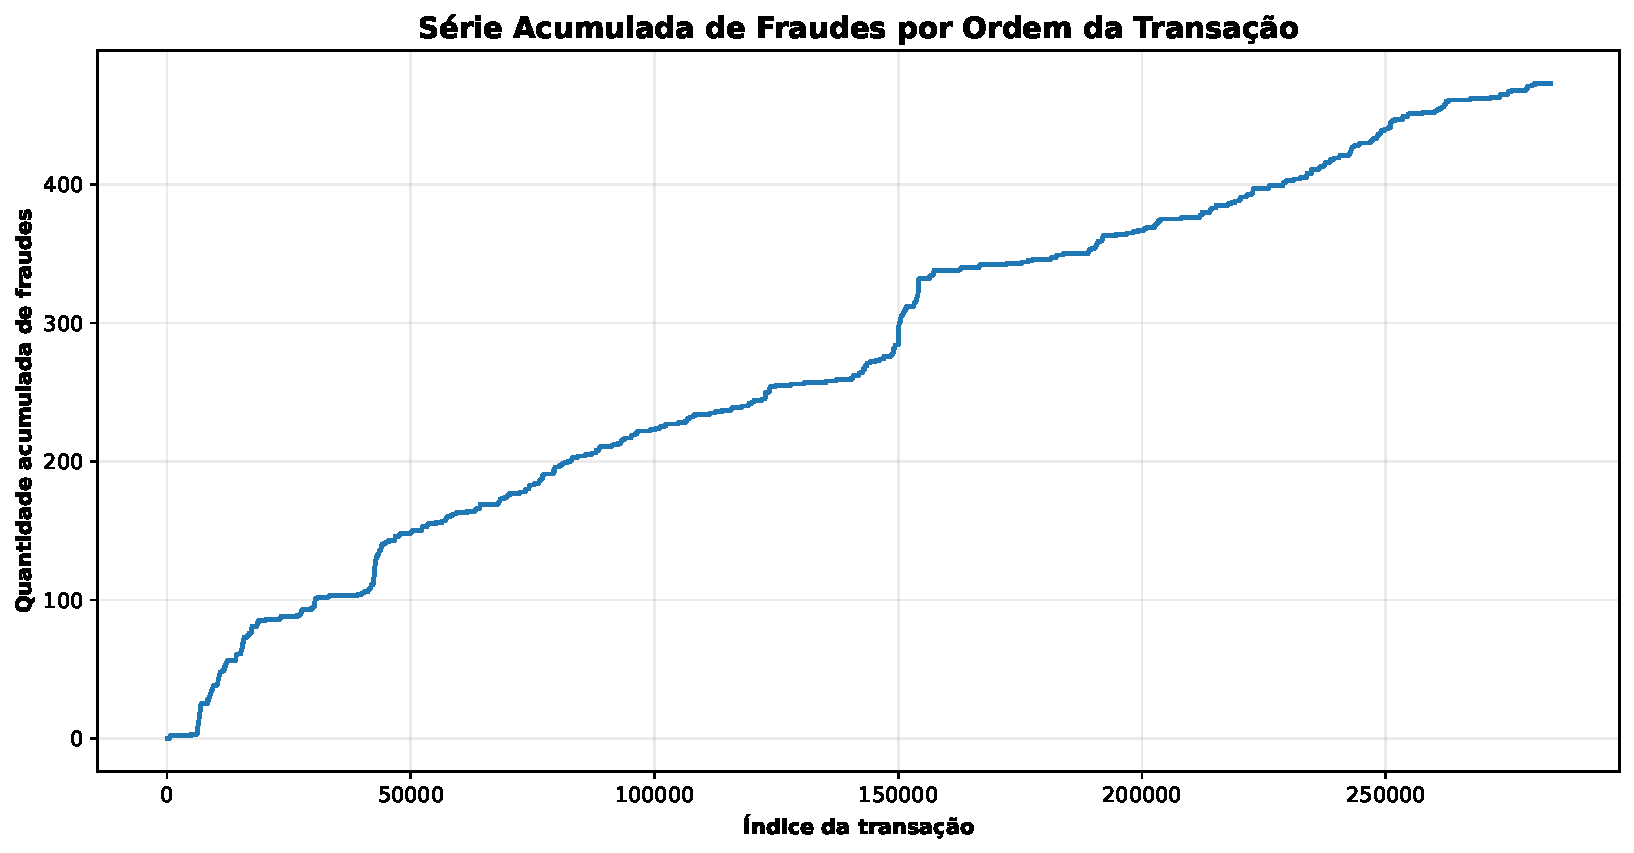
\includegraphics[width=\textwidth]{relatorio_target/grafico_serie_acumulada_fraudes.pdf}
\caption{Série acumulada de fraudes pela ordem das transações.}
\label{fig:target-serie-acumulada}
\end{figure}

\begin{figure}[H]
\centering
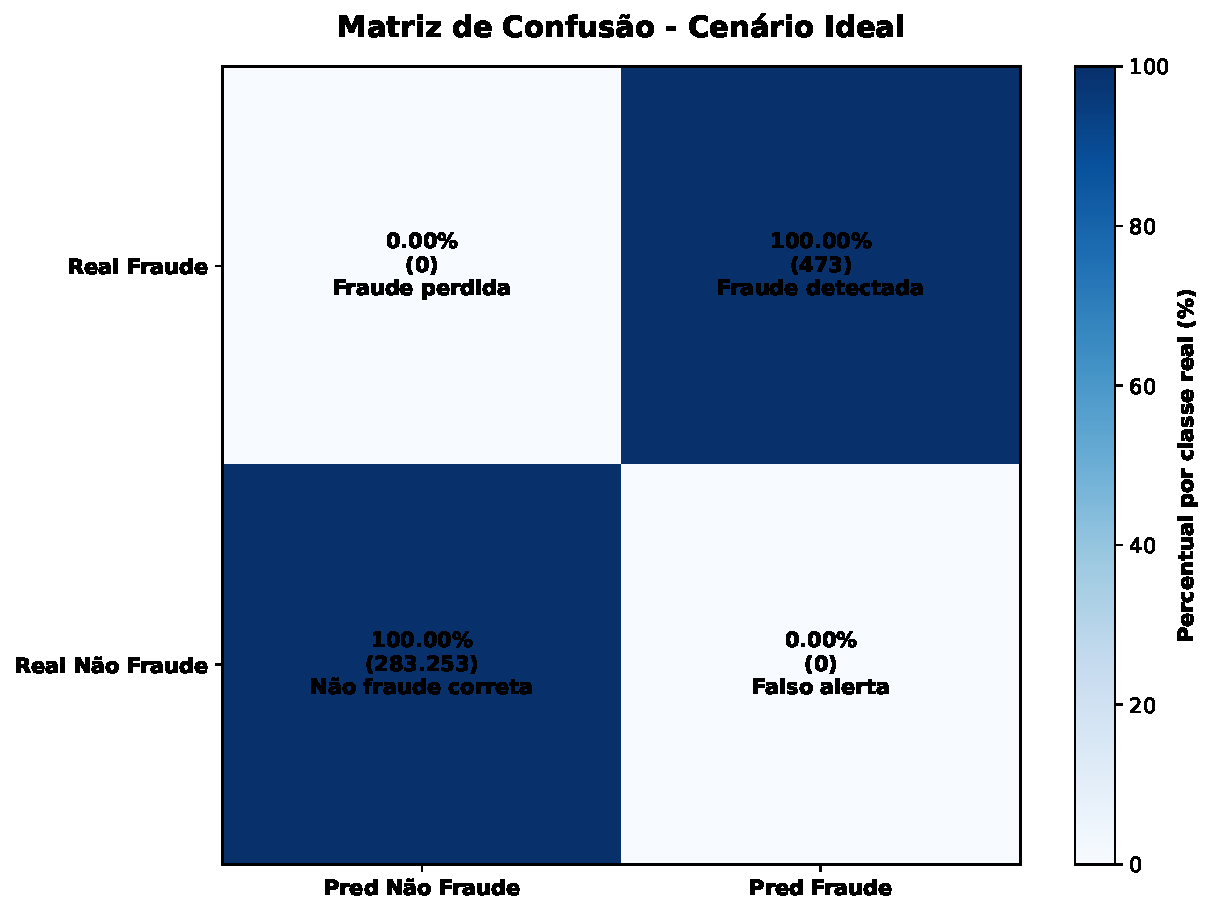
\includegraphics[width=0.85\textwidth]{relatorio_target/matriz_confusao_ideal.pdf}
\caption{Matriz de confusão do cenário ideal.}
\label{fig:matriz-target-ideal}
\end{figure}

\begin{figure}[H]
\centering
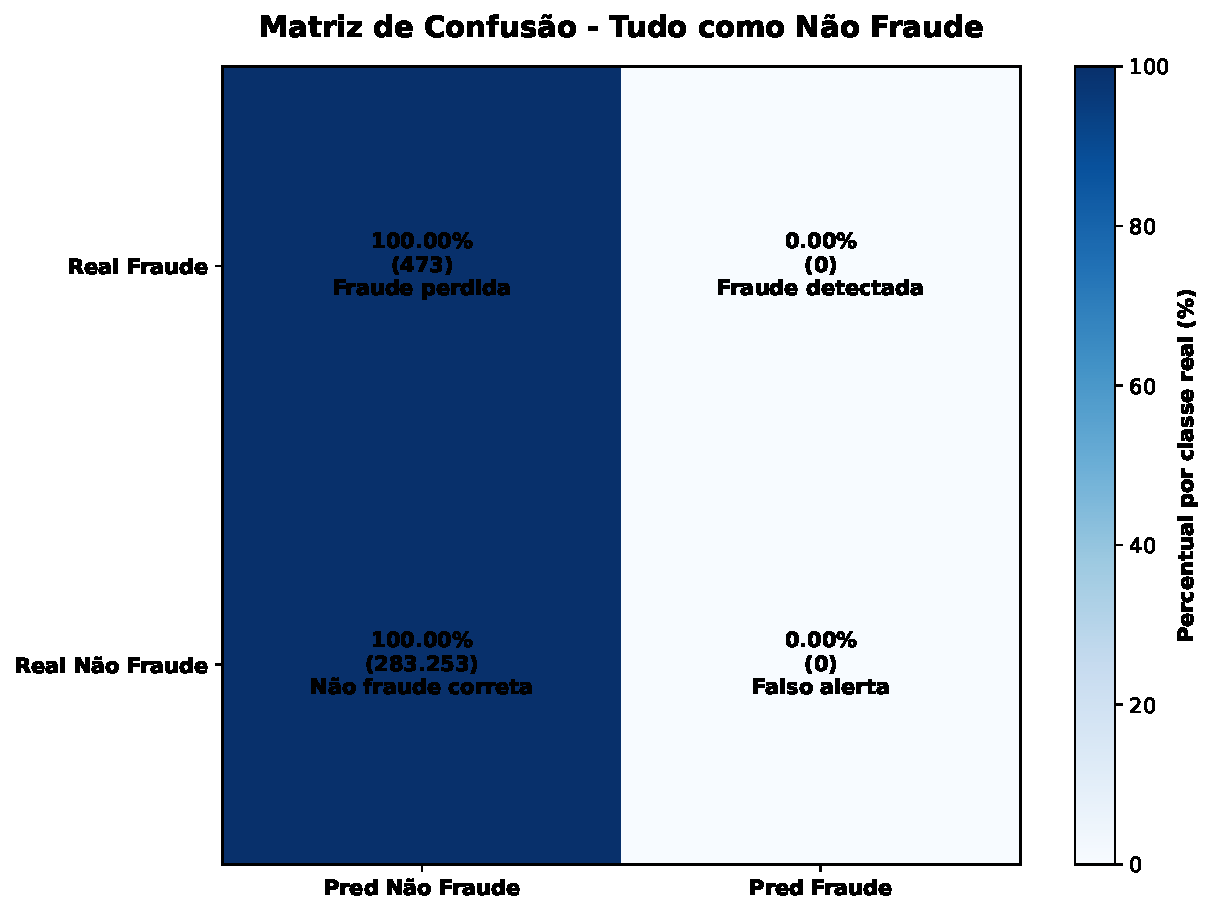
\includegraphics[width=0.85\textwidth]{relatorio_target/matriz_confusao_tudo_nao_fraude.pdf}
\caption{Matriz de confusão do baseline que classifica todas as transações como não fraude.}
\label{fig:matriz-target-tudo-nao-fraude}
\end{figure}

\begin{figure}[H]
\centering
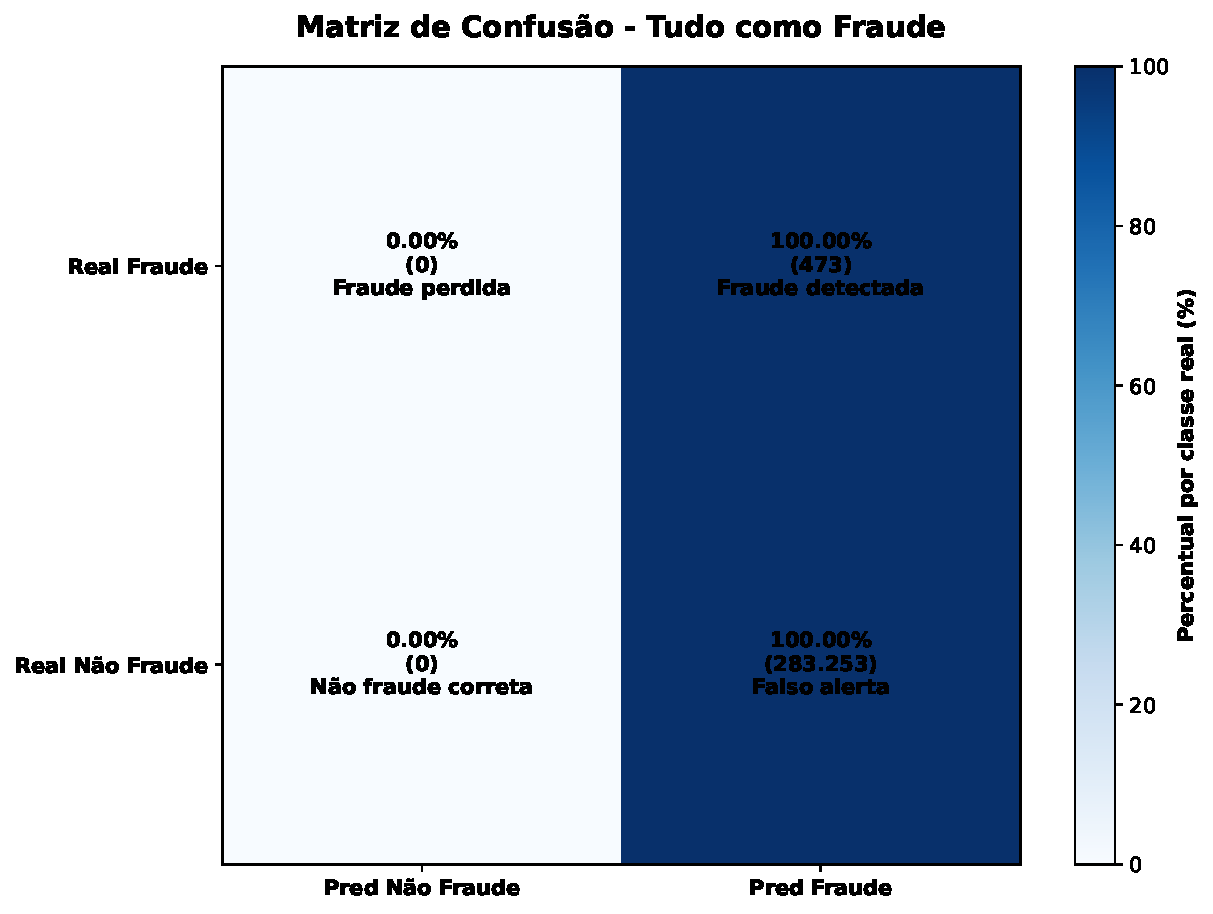
\includegraphics[width=0.85\textwidth]{relatorio_target/matriz_confusao_tudo_fraude.pdf}
\caption{Matriz de confusão do baseline que classifica todas as transações como fraude.}
\label{fig:matriz-target-tudo-fraude}
\end{figure}
